\chapter{Analyze Honeypot Attacks in the Cloud}
\label{chap:cloud-security}

Attacks from the Internet often originate from bots.
A bot, short for \enquote{robot}, is an automated process that interacts with different network services.
Besides good intentions, bots can be used for malicious purposes.
Mostly, bots try to self-propagate malware across the Internet and try to capture hosts that merge into a botnet \cite{Feily2009}.
Recently, Universities in Germany received more cyberattacks than ever, respectively increasing their costs for damage repairs.
Honeypots are a good solution to catch attackers and learn from their exploits.
However, it is not clear whether honeypots are an appropriate countermeasure to prevent such damage in the age of bots.
Following the rise of cyberattacks, this chapter introduces a method to collect and analyze cyberattacks in a cloud environment.
It further proposes an answer if honeypots are helpful to detect bot activities.

\section{Introduction}

As previously mentioned in \autoref{sec:cloud-computing}, using cloud resources is becoming the go-to option for new services and applications.
\citet{Kelly2021} thoroughly investigated honeypots on Azure, \ac{aws}, and \ac{gcp}.
Followingly, this chapter presents their results briefly to compare them with the ones heiCLOUD achieves.
The results are collected by T-Pot version $20.06.0$ for three weeks.
In addition, \citet{Kelly2021} considered different server geographical locations.
They have collected data from East US, West Europe, and Southeast Asia.
\autoref{tab:overview-cloud-security} shows the results presented by \citet{Kelly2021}.
Dionaea (a honeypot to capture malicious payload), Cowrie (\ac{ssh} and Telnet honeypot), and Conpot (industrial honeypot for \ac{ics}, and \ac{scada}) are the most attacked honeypots in comparison to the others.
Regarding \ac{aws}, Dionaea accounts for $91\%$ of the total attacks, Glutton and Cowrie are minor with $5\%$, and $2\%$.
Interestingly, Cowrie reported several attacks related to the COVID-19 pandemic to enable social engineering methods.
In contrast to \ac{aws}, Cowrie logged the majority of attacks with $51\%$ on \ac{gcp}.
Besides several automated attacks trying to log in with default credentials, adversaries tried to gather information about \ac{gpu} architecture, scheduled tasks, and privilege escalation.
Microsoft Azure reflects nearly the same results as the other two cloud providers beforehand.

\begin{table}
    \centering
    \caption[Overview of attacks on cloud providers]{
        Overview of attacks on cloud providers.
        For a better overview, only the three most attacked honeypots are listed.
        The others combine several honeypots.
    }
    \begin{tabularx}{\linewidth}{l|XXXX|l}
        \toprule
        \textsc{Provider} & \multicolumn{4}{c|}{\textsc{Honeypot}} & \textsc{In Total}                                                           \\
                          & \textbf{Dionaea}                       & \textbf{Cowrie}   & \textbf{Glutton} & \textbf{others}  &                   \\
        \hline
        \acl{aws}         & \numprint{228075}                      & \numprint{4503}   & \numprint{11878} & \numprint{3688}  & \numprint{248144} \\
        \acl{gcp}         & \numprint{162570}                      & \numprint{297818} & \numprint{84375} & \numprint{36403} & \numprint{581116} \\
        Microsoft Azure   & \numprint{308102}                      & \numprint{9012}   & \numprint{17256} & \numprint{6365}  & \numprint{340735} \\
        \bottomrule
    \end{tabularx}
    \label{tab:overview-cloud-security}
\end{table}

The overall results show an average ratio of \numprint{55000} attacks per day, summing up to roughly $1.17$ million in total.
Similar results for different regions could have been reproduced.
Their results clearly show the Europe, US, and Asia disparity.
An important question that \citet{Kelly2021} answered is if attackers target services on cloud providers based on the cloud providers' market share.
The study could not confirm this assumption because Google Cloud received most of the attacks with the smallest market share.
In total, most of the attacks are originated from Vietnam, Russia, the United States, and China.
Due to technologies such as \ac{vpn} or Tor, the geolocation only indicates the last node so that location data might be distorted.
Across all providers, roughly $80\%$ of the source \ac{ip} addresses had a bad reputation (identified by Suricata) and could have been filtered by the organization.
The operating devices used for attacking the services are mostly Windows 7 or 8 and different Linux kernels and distributions.
Windows devices target vulnerabilities in remote desktop sharing software.
Such vulnerabilities are
\begin{enumerate*}[label=(\roman*)]
    \item CVE-2006-2369\cite{CVE-2006-2369} (RealVNC\footnote{RealVNC is }) in the US region,
    \item CVE-2001-0540\cite{CVE-2001-0540} (\ac{rdp}) in EU and Asia regions,
    \item CVE-2012-0152\cite{CVE-2012-0152} (\ac{rdp}) in the Asia region, and
    \item CVE-2005-4050\cite{CVE-2005-4050} (\ac{voip}) in EU region
\end{enumerate*}.
In addition, attackers were also capable of disguising any fingerprinting activity of p0f.

This chapter compares the findings \citet{Kelly2021} claimed in the paper \enquote{A Comparative Analysis of Honeypots on Different Cloud Platforms} with ours using the Heidelberg University's cloud solution.
First, a short introduction of heiCLOUD is given, followed by a closer lookup of the T-Pot used to acquire data.
Lastly, it presents the results and does a thorough comparison closing up with a discussion based on a technical report of Cambridge University.

\section{Methodology}

The foremost goal is to track as many attacks as possible.
\autoref{fig:concept} sketches the concept to achieve this goal to gather various attacks from the Internet.
Honeypots should be deployed on a single instance, and their data or log files are stored in a database.
With the help of data visualization tools, the attacks are analyzed.
For security reasons, honeypots should run in a virtualized environment to avoid harming the host system.
The host machine runs on a Debian distribution.
The instance runs on heiCLOUD, a cloud service provided by Heidelberg University.
It is capable of 16 \ac{gb} of \ac{ram}, 8 \acp{vcpu}, and volatile memory of 30 \ac{gb}.
In addition, it mounts a 125 \ac{gb} permanent volume to store the data securely.
In the very early stage of this chapter, different approaches to achieve this goal have been compared.
For example, native implementation approaches, additional frameworks, and ready-to-use solutions have been evaluated.
However, the T-Pot, developed by Telekom, offers a profoundly ready-to-use solution with significant advantages.
It combines several honeypots with various analytic tools to trace the newest attacks.
Furthermore, it helps to compare the findings with the ones \citet{Kelly2021} claim.

\begin{figure}
    \centering
    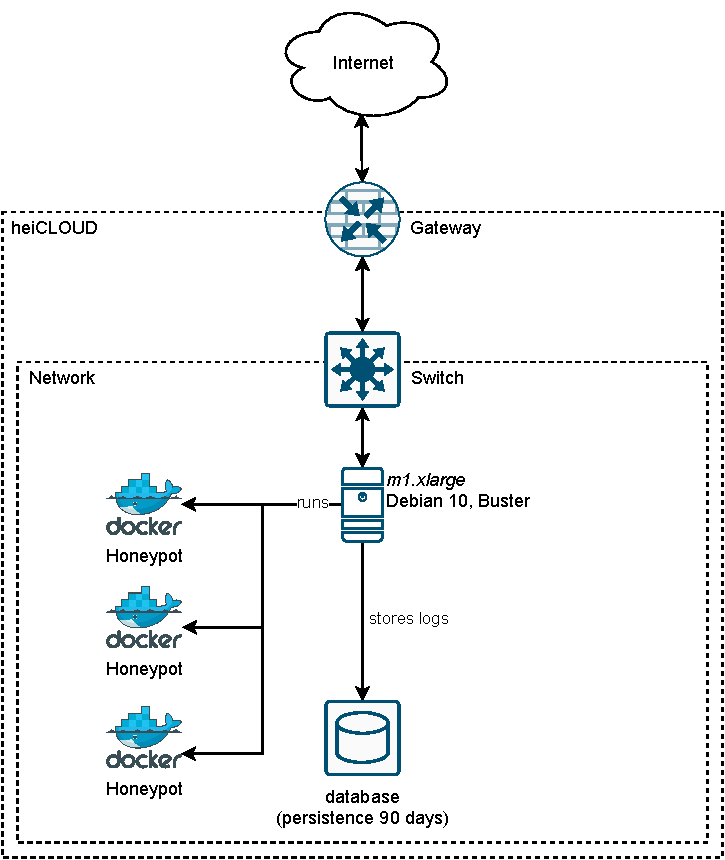
\includegraphics{figures/tpot-concept.pdf}
    \caption[Concept to collect honeypot attacks]{
        Concept to collect honeypot attacks.
        The instance size is referred to the available resources of OpenStack.
        The network is an encapsulated subnet with a switch for incoming and outgoing connections.
        The database is independent of the instance and could run on a separate host.
    }
    \label{fig:concept}
\end{figure}

Running the instance and exposing it to the Internet needs some adjustments beforehand.
Therefore, a virtual network with subnet \ipAddress{192.168.145.0/24} has been created wherein the \ac{ip} address \ipAddress{192.168.145.4} is assigned to the instance.
The instance is accessible from the outside with a floating \ac{ip} address \ipAddress{129.206.5.74}.
Access rules are similar to a stateless firewall, and thus, do not block any attacks.
Ports $1-64000$ are exposed and can be attacked by anyone.
Ports higher than $64000$ are only accessible through the university network \ipAddress{129.206.0.0/16} or eduroam \ipAddress{147.142.0.0/16} and should provide a basic authentication with username and password.

\subsection{heiCLOUD}
\label{subsec:heicloud}

\citet{urz2021} offers a \enquote{\ac{iaas} specially tailored for higher education and research institutions} called heiCLOUD.
It supplies multiple institutes at Heidelberg University with storage, virtual machines, or network components.
In addition, heiCLOUD is a DFN\footnote{German National Research and Education Network, the communications network for Science and research in Germany} member and offers others to use their services.
As stated on their information website\cite{heicloud2021}, it is
\begin{enumerate*}[label=(\roman*)]
    \item capable of freely manageable IT resources,
    \item beholds a stable and fast connection,
    \item ensures high availability and scalability,
    \item has freely selectable VM operating systems, and
    \item has a transparent payment model
\end{enumerate*} \cite{heicloud2021}.
Users can easily create their network areas and manage their space individually based on the open-source application OpenStack.
Unlike well-known cloud providers, heiCLOUD servers are located within Germany, thus, abide by the European data privacy law.
HeiCLOUD has never considered honeypots for additional cybersecurity measurements.

\subsection{T-Pot}
\label{subsec:tpot}

To be able to compare the results with \citet{Kelly2021}, the same approach to capture recent cyberattacks is used.
The T-Pot solution, a mixture of Telekom and Honeypot, stands out with its sheer quantity of various honeypots.
It requires at least $8$ \ac{gb} of \ac{ram} and a minimum of $128$ \ac{gb} of hard drive storage.
Based on a Debian 10 Buster distribution, it relies on Docker to run their services \cite{docker2021}.
T-Pot has to be deployed in a reachable network where intruders are expected.
Either \ac{tcp} and \ac{udp} traffic are forwarded without filtering to the network interface, or it runs behind a firewall with forwarding rules.
Specified ports for attackers are $1$-$64000$; higher ports are reserved for trusted IPs; thus, a reverse proxy asks for basic authentication.
All daemons and tools run on the same network interface, but some are encapsulated in their own Docker network.
The lightweight virtualization technology Docker uses containers to run on the host system \cite{combe2016}.
Unlike virtual machines, Docker reduces overhead with the downside of a greater attack surface.
To mitigate attacks, Docker wraps containers in an isolated environment.
This is achieved by restricting the kernel namespace and control groups (\verb|cgroups|).
\autoref{fig:overview-tpot} visualizes the technical concept of T-Pot.
Each service has dedicated ports or port ranges that are exposed.
Attackers can communicate either with \ac{tcp} or \ac{udp}.
All honeypots and tools create log files used to get any knowledge about attackers.
In order to view and trace current attacks, T-Pot uses the ELK stack.
ELK is the acronym of Elasticsearch, Logstash, and Kibana \cite{elastic2021}.
The search engine Elasticsearch is based on the Lucene library.
It is multitenant-capable and offers full-text search via \ac{http}.
Logstash is used to feed Elasticsearch.
In general, it offers an open server-side data processing pipeline that helps to send data from multiple sources to an Elasticsearch node.
Kibana is the primary data visualization tool.
It enables users to create plots and dashboards, crawl Elasticsearch, and trace the system's health.
All logs of the honeypots and tools are forwarded to the search engine Elasticsearch by Logstash.
The ELK stack is not directly exposed to the Internet; thus, authentication is unnecessary.
Users can monitor all log files with Kibana by pre-defined dashboards or custom search queries.
In addition, T-Pot features different services types, namely
\begin{enumerate*}[label=(\roman*)]
    \item standard,
    \item sensor,
    \item industrial,
    \item collector,
    \item next generation, and
    \item medical
\end{enumerate*}.
Each service type has a different set of honeypots and tools tailored to its core idea.
T-Pot feeds their data to an external Telekom service; however, this data submission can be turned off.
The latest version, $20.06.0$, has been used in this chapter.
Newer versions might be available by the end of this study and could differ from this.

\begin{sidewaysfigure}
    \centering
    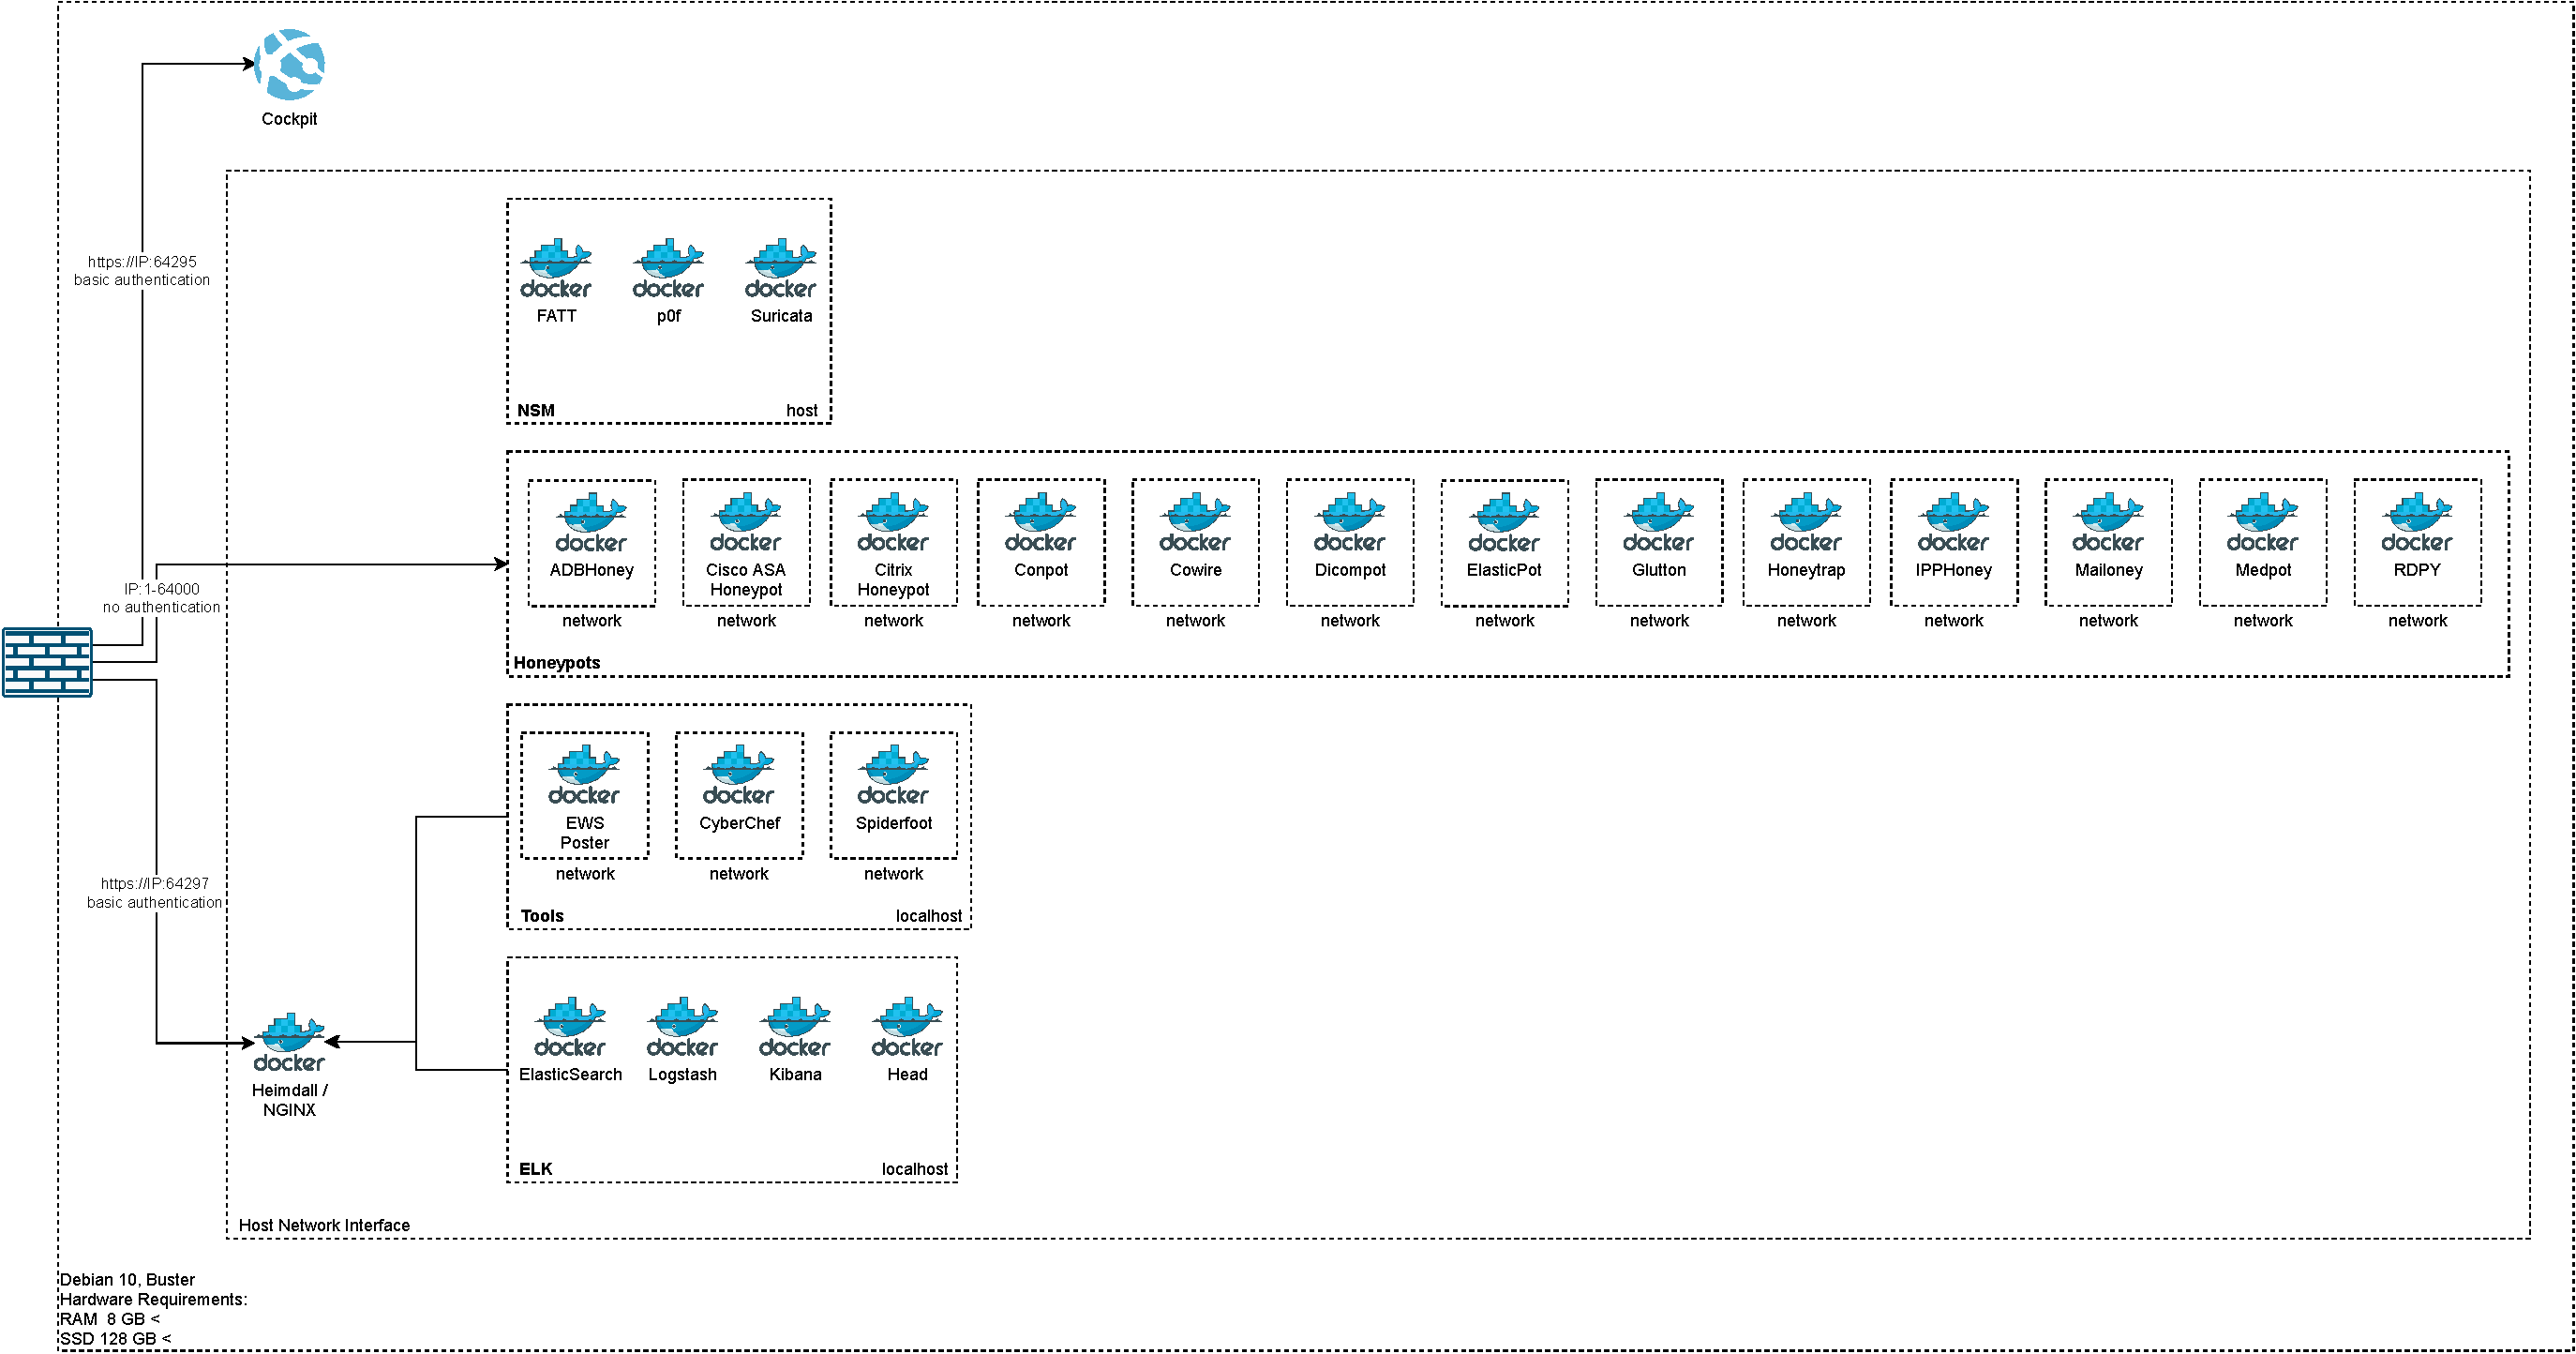
\includegraphics[width=\textwidth]{figures/tpot-architecture.pdf}
    \caption[T-Pot architecture]{
        T-Pot architecture derived from \cite{tpot2021}.
        Honeypots are encapsulated in their network.
        NSM runs on the host network, and thus, receives every packet.
        ELK and tools run on localhost and are accessible through NGINX.
        The Cockpit application is a web-based graphical interface for servers
    }
    \label{fig:overview-tpot}
\end{sidewaysfigure}

\subsubsection{Honeypots}

T-Pot consists of 20 honeypots.
Albeit the sheer quantity of it, a short explanation is given.
In addition, \autoref{tab:overview-honeypots} gives a quick overview of all available honeypots in conjunction with
\begin{enumerate*}[label=(\roman*)]
    \item the port they are running on,
    \item their interaction level, and
    \item a short description
\end{enumerate*}.

\textbf{ADBHoney} \cite{adbhoney2021} is a low-interaction \ac{adb} honeypot over \ac{tcp}/\ac{ip}.
The importance of it lies in the \ac{adb} protocol that is used for debugging and pushing content to an Android device.
However, unlike \ac{usb} connection, it does not support any kind of ample mechanisms of authentication and protection.
By exposing the \ac{adb} service over any port, an adversary could connect and exploit it.
ADBHoney is designed to catch malware that has been pushed onto devices.

\textbf{Cisco \ac{asa}} \cite{cymmetria2018} is a low-interaction honeypot that detects CVE-2018-0101\cite{CVE-2018-0101}.
It is a vulnerability that could allow an unauthenticated, remote attacker to cause a reload of the affected system and remotely execute code.
This can be achieved by flooding a webvpn-configured interface with crafted \ac{xml} packets.
Consequently, the attacker obtains full control by executing arbitrary code.

\textbf{Citrix \ac{adc} honeypot} \cite{citrixhoneypot2020} detects and logs CVE-2019-19781\cite{CVE-2019-19781} scans and exploitation attempts.
This vulnerability allows adversaries to perform directory traversal attacks.
Files are accessible by path strings to denote the file or directory.
In addition, some file systems include special characters to traverse the hierarchy easily.
Attackers take advantage of it by combining special characters to get access to restricted areas. \cite{flanders2019}

\textbf{Conpot} \cite{conpot2021} is a low-interaction industrial honeypot for \ac{ics}, and \ac{scada}.
It provides a variety of different standard industrial control protocols.
An adversary should be tricked by the complex infrastructure and lured into attacks.
In addition, a custom human-machine interface can be connected to increase the attack surface.
By randomly delaying the response time, Conpot tries to emulate a real machine handling a certain amount of load.

\textbf{Cowrie} \cite{cowrie2021} is a medium- to high-interaction \ac{ssh} and Telnet honeypot.
It offers to log brute-force attacks and shell interactions with attackers.
In medium-interaction mode, Cowrie emulates a UNIX shell in Python, whereas in high-interaction mode, it proxies all commands to another system.

\textbf{DDoSPot} \cite{ddosspot2021} is a low-interaction honeypot to log and detect \ac{udp}-based \ac{ddos} attacks.
It is a platform used to support various plugins for different honeypot services and servers.
Currently, it supports \ac{dns}, \ac{ntp}, \ac{ssdp}, \ac{chargen}, and random/mock \ac{udp} server.

\textbf{Dicompot} \cite{dicompot2021} is a low-interaction honeypot for the \ac{dicom} protocol.
As with other honeypots before, it mocks a \ac{dicom} server in Go to collect logs and detect attacks.

\textbf{Dionaea} \cite{dionaea2021} is a medium-interaction honeypot that tries to capture malware copies by exposing services.
It supports various protocols such as \ac{ftp}, \ac{smb}, and \ac{http}.
Several modules can be integrated to work with Dionaea for further malware results, such as VirusTotal.

\textbf{Elasticpot} \cite{elasticpot2021} is a low-interaction honeypot for Elasticsearch, a search engine based on the Lucene library.

\textbf{Glutton} \cite{glutton2021} is a generic low-interaction honeypot that works as a \ac{mitm} for \ac{ssh} and \ac{tcp}.
However, lacking documentation does not provide a deeper insight into this honeypot.

\textbf{Heralding} \cite{heralding2021} is a credential catching honeypot for protocols like \ac{ftp}, Telnet, \ac{ssh}, \ac{http}, or \ac{imap}.

\textbf{HoneyPy} \cite{honeysap2021} is a low to medium-interaction honeypot that supports several protocols such as UDP or \ac{tcp}.
New protocols can be added by writing a custom plugin for them.
HoneyPy gives the freedom of quickly deploying and extending honeypots.

\textbf{HoneySAP} \cite{honeysap2021} is a low-interaction honeypot tailored for SAP services.

\textbf{Honeytrap} \cite{honeytrap2021} is a low-interaction honeypot network security tool.
As stated by \citet*{honeytrap2021}, Honeytrap is vulnerable to buffer overflow attacks.

\textbf{IPPHoney} \cite{ipphoney2021} is a low-interaction \ac{ipp} honeypot.

\textbf{Mailoney} \cite{mailoney2021} is a low-interaction \ac{smtp} honeypot written in Python.

\textbf{MEDpot} \cite{medpot2021} is a low-interaction honeypot focused on \ac{fhir}.
It is a standard description data format to transfer and exchange medical health records.

\textbf{RDPY} \cite{rdpy2021} is a low-interaction honeypot of the Microsoft \ac{rdp} written in Python.
It features client and server-side, and it is based on the event-driven network engine Twisted.
It supports authentication over \ac{tls} and \ac{nla}.

\textbf{SNARE and TANNER} \cite{snare2021, tanner2021} is a honeypot project.
SNARE is an abbreviation for Super Next-generation Advanced Reactive honEypot.
It is a successor of Glastopf, a web application sensor.
In addition, it supports the feature of converting existing web pages into attack surfaces.
TANNER \cite{tanner2021} can be seen as SNARES' brain.
Whenever a request has been sent to SNARE, TANNER decides how the response should be.

\subsubsection{Tools}

T-Pot integrates tools to screen network traffic and block DoS attacks.

\textbf{FATT} \cite{fatt2021} is used to extract metadata and fingerprints such as JA3 \cite{ja32021} and HASSH \cite{hassh2021} from captured packets.
JA3 is a method for \enquote{creating SSL/TLS client fingerprints} whereas HASSH is a network fingerprinting standard that is used to identify specific client and server \ac{ssh} implementations.
In addition, it features live network traffic.
As noted by the author, FATT is based on a python wrapper for tshark, namely pyshark, and thus has performance downturns.
T-Pot applies FATT on every request made on the host network.

\textbf{Spiderfoot} \cite{spiderfoot2021} is an open-source intelligence automation tool that helps to screen targets to get information about what is exposed over the Internet.
It can target different entities such as \ac{ip} address, domain, hostname, or network subnet.
In addition, it features more than 200 modules that can be integrated as an extension.
T-Pot uses it to scan defensively and thus not include any other module.

\textbf{Suricata} \cite{suricata2021} is \enquote{a high performance \ac{ids}, \ac{ips} and \ac{nsm} engine}.
T-Pot lets Suricata analyze and assess any request made on the host network.

\textbf{P0f} \cite{p0f2021} is a fingerprinting tool that uses passive traffic fingerprinting mechanisms to check \ac{tcp}/\ac{ip} communications.
T-Pot lets p0f passively check any request made on the host network.

\textbf{Endlessh} \cite{endlessh2021} is an \ac{ssh} server that sends an endless, random \ac{ssh} banner.
The key idea is to lock up \ac{ssh} clients that try to connect to the \ac{ssh} server.
It lowers the transaction speed by intentionally inserting delays.
Due to the established connection before the cryptographic exchange, this module does not require any cryptographic libraries.

\textbf{HellPot} \cite{hellpot2021} is an \enquote{endless honeypot}.
If someone connects to this honeypot, it results in a memory overflow.
Its key idea is to send an endless data stream to the attacker until its memory or storage runs out.

\begin{sidewaystable}
    \centering
    \caption[Overview of honeypots of T-Pot]{
        Overview of all available honeypots of T-Pot with interaction level, port, and a short description.
        Ports are marked with either \ac{tcp} or UDP; if a port misses any definition, both \ac{tcp} and UDP are allowed.
    }
    \begin{tabularx}{\linewidth}{l|XlX}
        \toprule
        \textsc{Honeypots}                        & \multicolumn{3}{c}{}                                                                                                                                                                                                            \\
                                                  & \textbf{Port}                                                                                               & \textbf{Interaction-level} & \textbf{Description}                                                                 \\
        \hline
        ADBHoney \cite{adbhoney2021}              & 5555/TCP                                                                                                    & low                        & \ac{adb} protocol honeypot                                                           \\
        Cisco ASA \cite{cymmetria2018}            & 5000/UDP, 8443/TCP                                                                                          & low                        & honeypot for CVE-2018-0101\cite{CVE-2018-0101} detection                             \\
        Citrix honeypot \cite{citrixhoneypot2020} & 443/TCP                                                                                                     & low                        & detects and logs CVE-2019-19781\cite{CVE-2019-19781} scans and exploitation attempts \\
        Conpot \cite{conpot2021}                  & 80, 102, 161, 502, 623, 1025, 2404, \newline 10001, 44818, 47808, 50100                                     & low                        & industrial honeypot for \ac{ics}, and \ac{scada}                                     \\
        Cowrie \cite{cowrie2021}                  & 2222, 23                                                                                                    & high                       & \ac{ssh} and Telnet honeypot                                                              \\
        DDoSPot \cite{ddosspot2021}               & 1112/TCP                                                                                                    & low                        & log and detect UDP-based \ac{ddos} attacks                                           \\
        Dicompot \cite{dicompot2021}              & 1112/TCP                                                                                                    & medium                     & honeypot for the \ac{dicom} protocol                                                 \\
        Dionaea \cite{dionaea2021}                & 21, 42, 69/UDP, 8081, 135, 443, 445, \newline 1433, 1723, 1883, 1900/UDP, \newline 3306, 5060/UDP, 5061/UDP & low                        & capture malware copies                                                               \\
        Elasticpot \cite{elasticpot2021}          & 9200                                                                                                        & low                        & honeypot for Elasticsearch                                                           \\
        Glutton \cite{glutton2021}                & NFQ                                                                                                         & medium                     & MitM proxy for \ac{ssh} and TCP                                                           \\
        Heralding \cite{heralding2021}            & 21, 22, 23, 25, 80, 110, 143, 443, \newline 993, 995, 1080, 5432, 5900                                      & low                        & credential catching honeypot                                                         \\
        HoneyPy \cite{honeysap2021}               & 7, 8, 2048, 2323, 2324, 4096, 9200                                                                          & low                        & extendable honeypot                                                                  \\
        HoneySAP \cite{honeysap2021}              & 3299/TCP                                                                                                    & low                        & honeypot for SAP services                                                            \\
        Honeytrap \cite{honeytrap2021}            & NFQ                                                                                                         & medium                     & captures attacks via unknown protocols                                               \\
        IPPHoney \cite{ipphoney2021}              & 631                                                                                                         & low                        & \ac{ipp} honeypot                                                                    \\
        Mailoney \cite{mailoney2021}              & 25                                                                                                          & low                        & SMTP honeypot                                                                        \\
        MEDpot \cite{medpot2021}                  & 2575                                                                                                        & low                        & \ac{fhir} honeypot                                                                   \\
        RDPY \cite{rdpy2021}                      & 3389                                                                                                        & low                        & Microsoft \ac{rdp} honeypot                                                          \\
        SNARE/TANNER \cite{snare2021}             & 80                                                                                                          & low                        & web application honeypot                                                             \\
        \bottomrule
    \end{tabularx}
    \label{tab:overview-honeypots}
\end{sidewaystable}

\section{Results}
\label{sec:honeypots-heicloud}

The T-Pot has been deployed for three weeks (from 26th of September to 16th of October) and collected in total \numprint{607747} attacks.
Overall, RDPY ($46.08\%$), Honeytrap ($33.23\%$), and Cowrie ($12.42\%$) received most of the attacks with a total amount of \numprint{540398} attacks.
\autoref{fig:overview-attacks} shows the distribution of honeypot attacks.
The total numbers are based on \autoref{tab:overview-honeypots-attacks}.

\begin{figure}
    \centering
    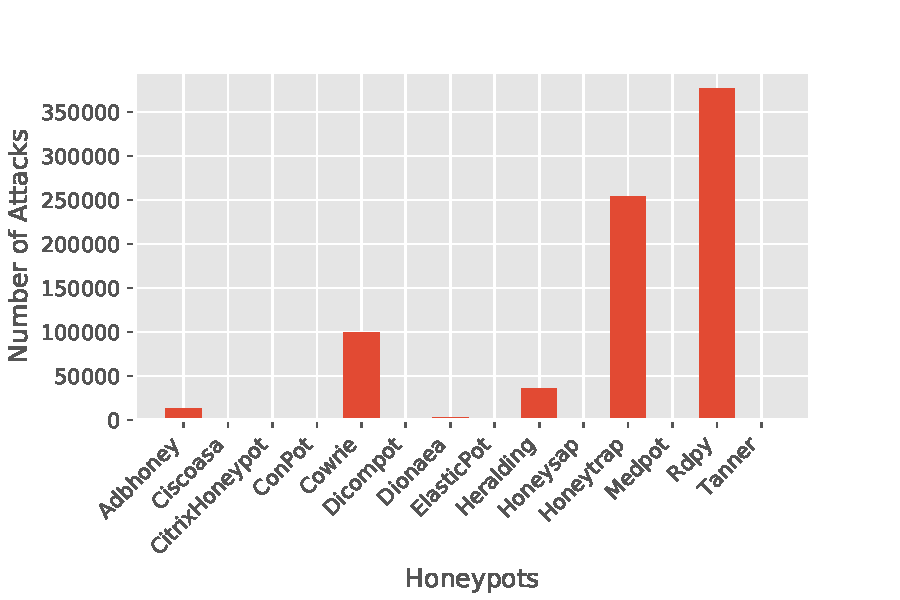
\includegraphics[width=\textwidth]{figures/tpot-overview-attacks.pdf}
    \caption[Distribution of honeypot attacks]{
        Distribution of honeypot attacks.
        Timestamp; 26th of September to 16th of October.
    }
    \label{fig:overview-attacks}
\end{figure}

% ====================================================================================================================
% Dionaea
What is striking is the large disparity between the previously mentioned attacks on \ac{aws}, \ac{gcp}, and Azure.
Especially with the honeypot Dionaea, it is unclear why only \numprint{2368} attacks have been performed.
$96\%$ of \ac{ip} addresses connected to Dionaea are known attackers, and $70\%$ were acquired on port 81, unofficially known for Tor routing.
Neither any malware nor suspicious payload could be identified.
An assumption is that the packets run through a static filter.
Heidelberg has a centralized stateless firewall, indicating that specific ports or protocols are excluded.
A \textsc{nmap} \ac{tcp} SYN scan (\verb|nmap -sS -A 129.206.5.74|) has been performed to prove this assumption that ports are excluded.
The result clearly shows that port 139 for \ac{smb} is filtered, although the access security explicitly allows it.
The stateless firewall runs in front of heiCLOUD and filters many ports, including $113$.
Based on this, it can be assumed that most of the attacks on Dionaea are carried out via \ac{smb}, which would explain the total number of attacks.
The administrator of the university firewall had been consulted to exclude the T-Pot instance to validate if the actual number is even higher without any packet filter in front of it.
Respectively, no stateless packet filter has been applied to the T-Pot for three weeks (2nd of December until 23rd of December).
It could identify a drastic increase in Dionaea attacks with a total number of \numprint{213053}.
Overall, $93\%$ of all attacks are on the smbd protocol followed by many database protocols such as mongod and mssqld.
This confirms the assumption that a higher total number of attacks would be the result without the packet filter in front of the instance.

Comparing the number with \citet{Kelly2021} it shows that Dionaea attacks surpass every other cloud provider.
However, Dionaea attacks will not be included in later results because usually, a server is not allowed to be excluded from the university firewall.
Only for this research purpose to assess the effect of the packet filter has an exclusion been granted.

\begin{figure}
    \centering
    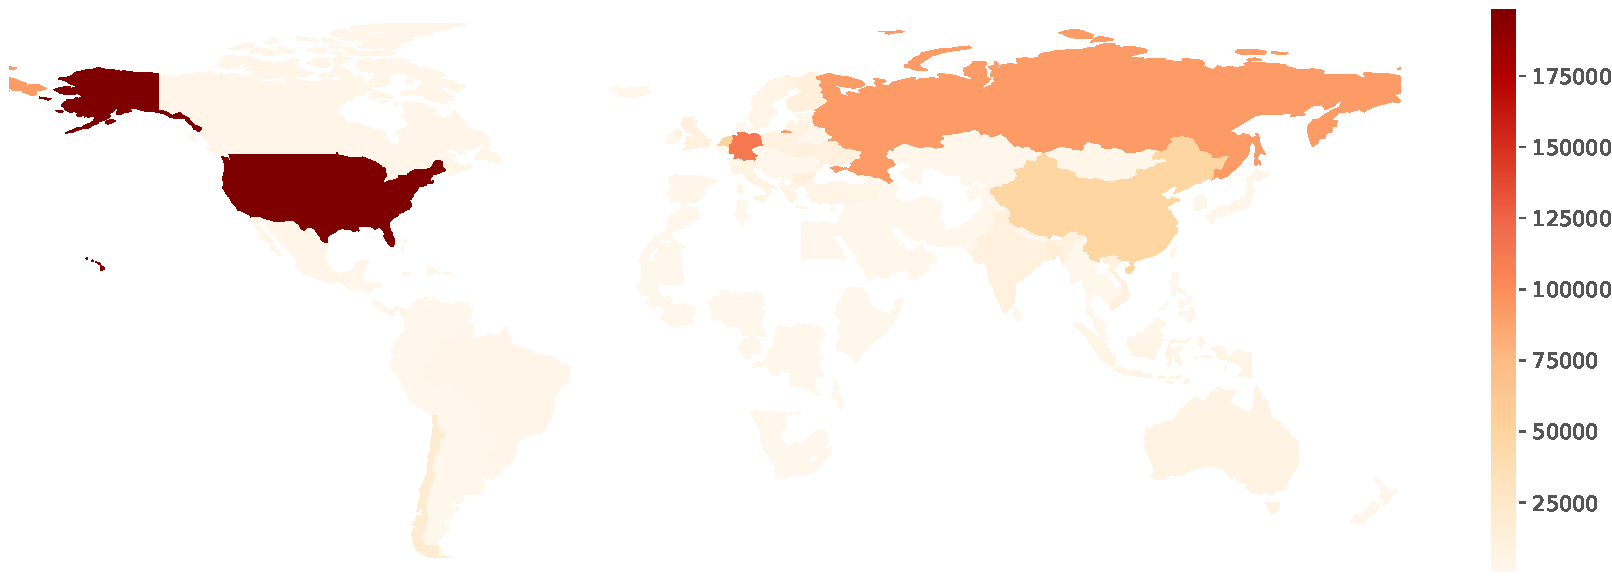
\includegraphics[width=\textwidth]{figures/tpot-overview-map.pdf}
    \caption[Attack distribution of T-Pot]{
        Attack distribution of T-Pot.
        The USA, Russia, China, and Germany are the most attacking countries.
        Timestamp; 26th of September to 16th of October.
    }
    \label{fig:attack-distribution}
\end{figure}

% ====================================================================================================================
% Location
Logstash uses GeoLite2 to resolve the source \ac{ip} address with information such as location, \ac{asn}, continent code, country name, and \ac{as} organization.
\autoref{fig:attack-distribution} indicates the geographical location of connections acquired to any honeypot.
Most attacks are originated from the United States, Germany, Russia, and China.
Large security scans of DFN or \ac{belwue} pushes Germany to second place; therefore, Germany can be considered negligible.
On the contrary, the geographical location of an \ac{ip} address merely indicates the true origin.
Due to technologies like \ac{vpn} or Tor, the last known node of an \ac{ip} address could be spoofed, and thus as stated by \citet{Kelly2021}, would remain insufficient to use.
Hence, no one should rely on geographical information.

\begin{figure}
    \centering
    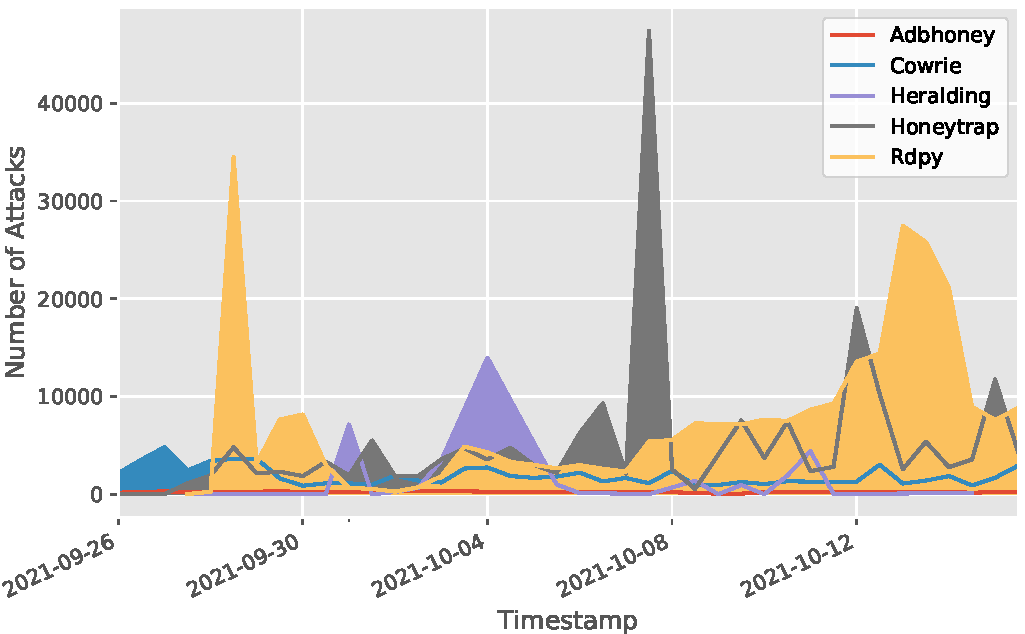
\includegraphics[width=\textwidth]{figures/tpot-attacks-histogram.pdf}
    \caption[Attack histogram of T-Pot]{
        Attack histogram of T-Pot.
        Only the five most attacked honeypots are considered.
        Timestamp; 26th of September to 16th of October.
    }
    \label{tpot-overview-histogram}
\end{figure}

Attacks are not equally distributed among all honeypots, and thus, different protocols and applications receive more attention than others.
\autoref{tpot-overview-histogram} shows the timeline of attacks that are executed on our instance separated by honeypots.
RDPY, Honeytrap, and Cowrie are the most attacked honeypots.
The high peak of Honeytrap in the middle indicates a full \textsc{nmap} scan from Germany that has been done to get an insight of the packet filtering at the Heidelberg University.
It identifies a bias towards remote desktop protocol attacks, shell-code exploitations, and commands to retrieve information about the \ac{cpu}, scheduled tasks (\verb|cat /proc/cpuinfo|, or \verb|crontab|), or privilege escalation.

\begin{figure}
    \centering
    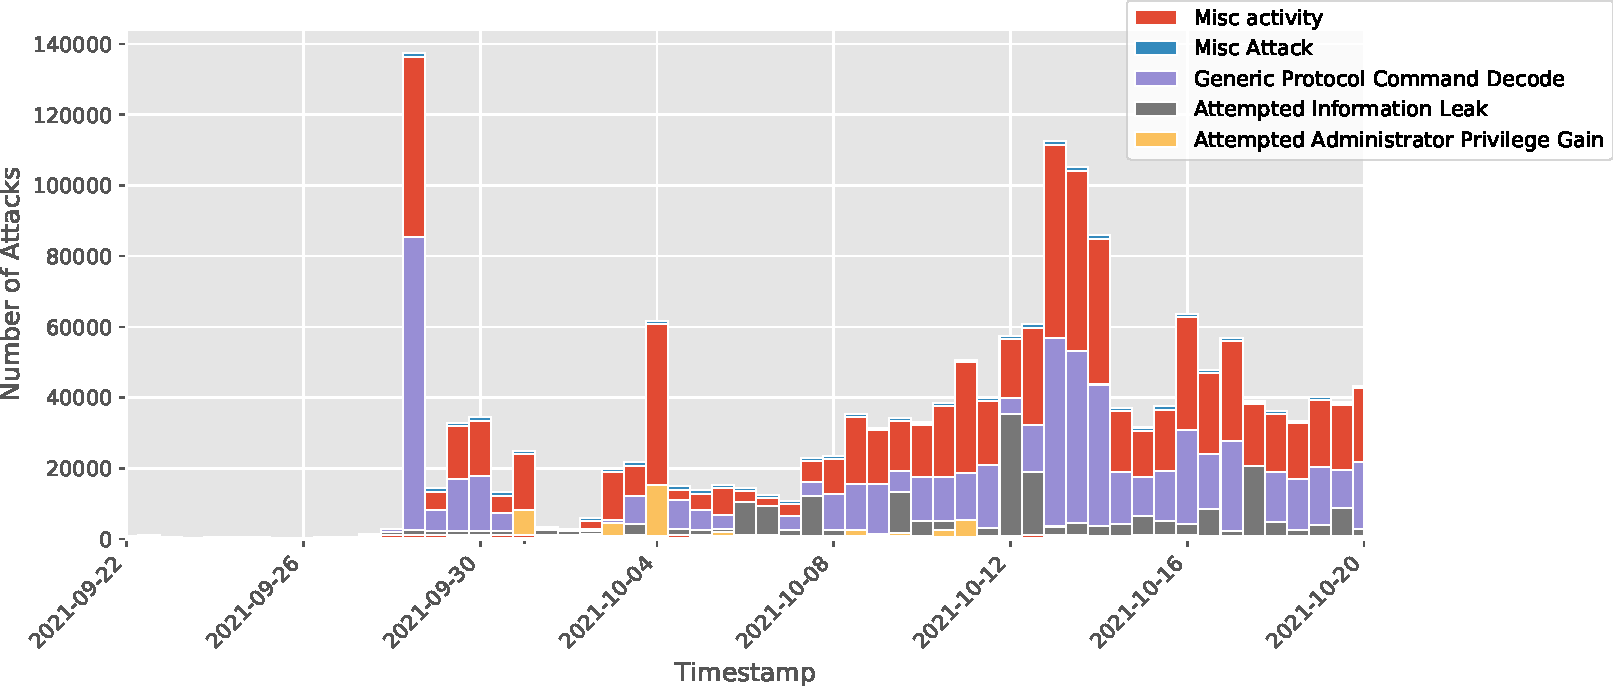
\includegraphics[width=\textwidth]{figures/tpot-suricata-alerts.pdf}
    \caption[Suricata results of T-Pot]{
        Suricata results of T-Pot.
        Displays the five most listed alert categories.
        Timestamp; 26th of September to 16th of October.
    }
    \label{fig:suricata-results}
\end{figure}

% ====================================================================================================================
% Suricata
Suricata registered several alerts and \acsp{cve}.
The vast majority of alerts are \ac{rdp}-related policies, \ac{vnc} authentication failures, and \textsc{nmap} scans.
Most used vulnerabilities are
\begin{enumerate*}[label=(\roman*)]
    \item CVE-2001-0540\cite{CVE-2001-0540} which is a memory leak in terminal servers in Windows NT and Windows 2000 causing a denial of service (memory exhaustion) by malformed \ac{rdp} requests,
    \item CVE-2006-2369\cite{CVE-2006-2369} which is a RealVNC vulnerability allowing hackers to bypass authentication, and
    \item CVE-2012-0152\cite{CVE-2012-0152} which enables attackers for \ac{rdp} in Microsoft Windows Server 2008 R2 and R2 SP1 and Windows 7 Gold and SP1 to cause a denial of service by sending a series of crafted packets
\end{enumerate*}.
As derived from \autoref{fig:suricata-results}, the T-Pot has not received many attacks in the first week.
Starting from the 28th of September, the number of alerts is skyrocketing.
This would indicate that bots crawl \ac{ip} address ranges to find new machines and probe them.
Interestingly, zero-day exploits like the Apache vulnerability \cite{CVE-2021-42013} that came with version $2.49.0$ got registered in CVE on the 6th of October and immediately recognized by Suricata on the 15th of October.
Attackers could perform a remote code execution using path traversal attacks when the \ac{cgi} scripts of Apache are enabled.
The logs could trace back similar attacks like \verb|/cgi-bin/.\%2e/\%2e\%2e/bin/sh| until the 7th of October, leaving an even smaller time frame to adapt to new exposures.
This shows how fast bots adapt to new vulnerabilities to compromise more systems.

\begin{figure}
    \centering
    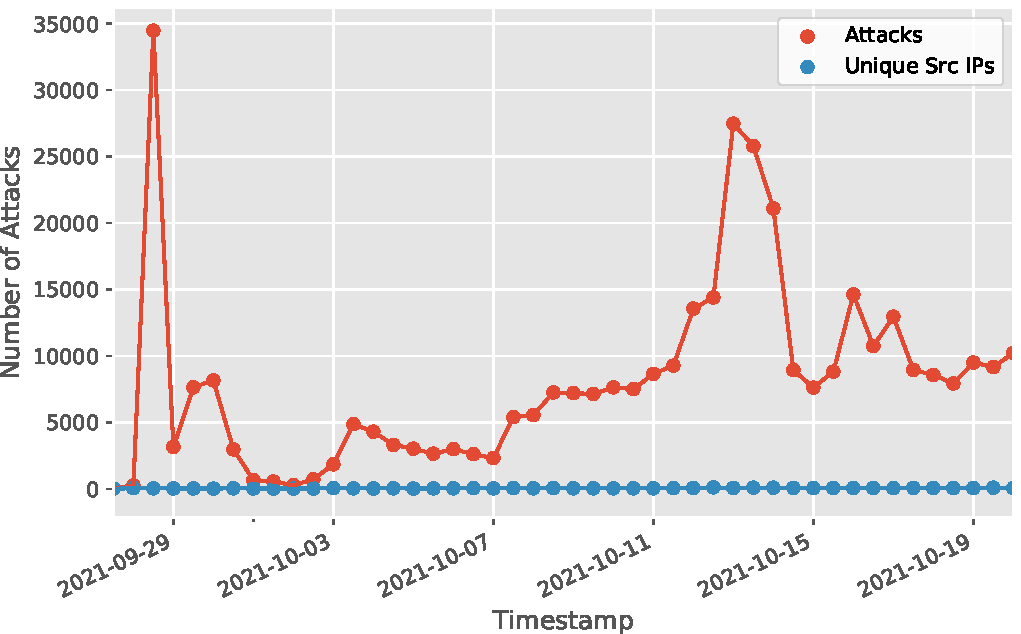
\includegraphics[width=\textwidth]{figures/tpot-rdpy-port.pdf}
    \caption[RDPY results of T-Pot]{
        RDPY attacks are separated into attacks and unique source \ac{ip} addresses.
        Timestamp; 26th of September to 16th of October.
    }
    \label{fig:rdpy-results}
\end{figure}

% ====================================================================================================================
% RDPY
The results from RDPY in \autoref{fig:rdpy-results} backups the assumption that attacks originate from bots.
It shows that only a small margin represents unique source \ac{ip} addresses.
The rest of the attacks result in either a bad reputation, bot, crawler, or known attacker.
\autoref{fig:suricata-results} shows the distribution of alert categories that Suricata identified.
Respectively, misc activities sum up to roughly $1.5$ million entries, \ac{rdp} related alerts account for two-thirds of it.
Several \ac{rdp} attacks from 2021 back to 2001 had been executed on the T-Pot.
Respectively, CVE-2012-0152 and CVE-2001-0540 coincide with the ones \citet{Kelly2021} claim.

\begin{figure}
    \centering
    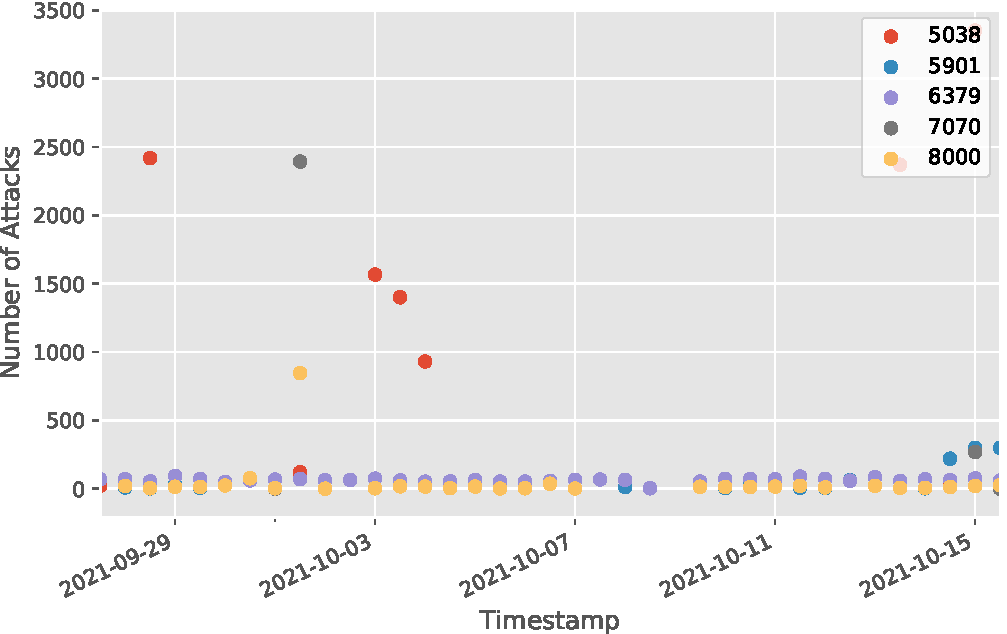
\includegraphics[width=\textwidth]{figures/tpot-honeytrap-port.pdf}
    \caption[Honeytrap results of T-Pot]{
        Honeytrap results of T-Pot.
        Timestamp; 26th of September to 16th of October.
    }
    \label{fig:honeytrap-results}
\end{figure}

% ====================================================================================================================
% Honeytrap
For NFQ related attacks, Honeytrap could identify three major services that are not provided by default.
Honeytrap functions as a honeypot to provide a service on ports that are not specified by default.
NFQ intercepts incoming \ac{tcp} connections during the \ac{tcp} handshake, and Honeytrap provides a service for it.
Most of these interceptions are made on
\begin{enumerate*}[label=(\roman*)]
    \item port 5038, which is used by a machine learning database called MLDB,
    \item port 5905, which an Intel Online Connect Access uses on Windows machines, and
    \item port 7070 which is used by Apple's QuickTime streaming server (RTSP)
\end{enumerate*}.
Nearly all ports attacks focused on \ac{rdp} connection attempts (\verb|Cookie: mstshash=Administr|).
However, $94\%$ of all connected \ac{ip} addresses on Honeytrap are resolved as known attackers.

\begin{figure}
    \centering
    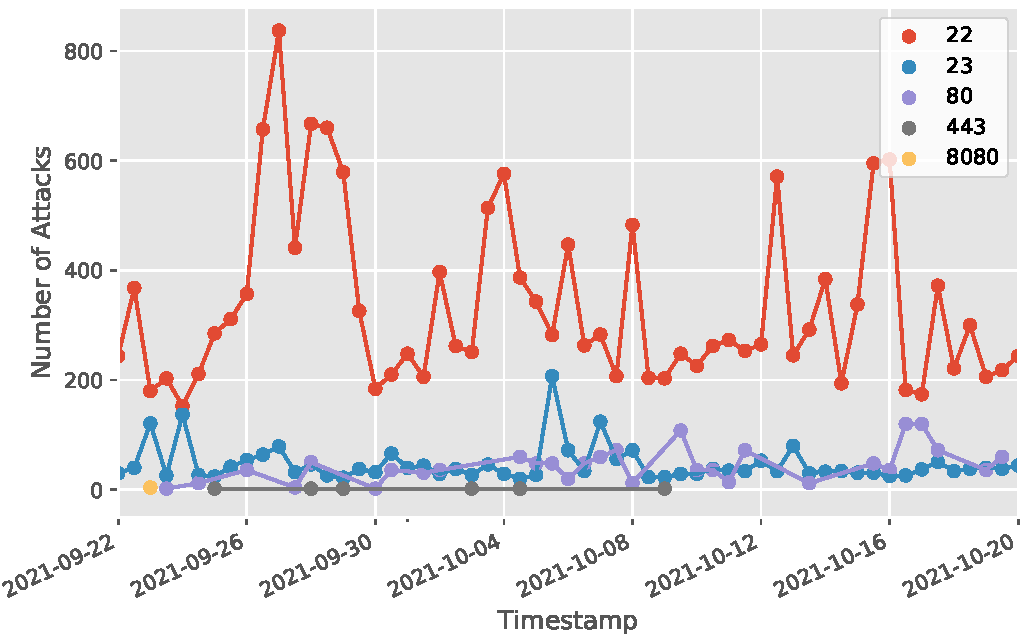
\includegraphics[width=\textwidth]{figures/tpot-cowrie-port.pdf}
    \caption[Cowrie results of T-Pot]{
        Cowrie results of T-Pot.
        Timestamp; 26th of September to 16th of October.
    }
    \label{fig:cowrie-results}
\end{figure}

% ====================================================================================================================
% Cowrie
The third most compromised honeypot is Cowrie, with a strong bias towards \ac{ssh} and \ac{ftp}.
\autoref{fig:cowrie-results} shows all attacks executed on Cowrie separated by their port.
Respectively, \ac{ssh} port $22$ is the most considered port, resulting in high use for privilege escalation.
Besides using default credentials to log in (\verb|username: root|, \verb|password: root|, see \autoref{fig:cowrie-credentials} for top 10 credentials), adversaries used various commands to retrieve any information about the host system (\verb|nproc;uname -a|, \verb|cat /proc/cpuinfo|).
A unique information gathering attack could be identified that has been widely used on the T-Pot.
\autoref{lst:code-exploitation} shows all shell commands that are executed.
Attackers try to gain knowledge about running processes on the system (\verb|/bin/busybox|).
Interestingly, crypto mining attacks are getting more attractive to criminals.
For example, XMRig has been the most downloaded malware for cryptocurrency mining.
Some adversaries even executed complex tailored shell commands to exploit the host machine as a crypto miner (\autoref{lst:crypto-exploitation}).
It is not surprising that such attacks gain attraction concerning the current time.
Attackers could exploit machines for crypto mining in order to earn more money.
This looks more appealing than acquiring mining machines and hijacking electricity from surrounding apartments.

\begin{figure}
    \lstinputlisting[language=bash, caption={[Cowrie attack to gather various information about the system]Cowrie attack to gather various information about the system.}, label={lst:code-exploitation}]{listings/exploit-cpu.sh.txt}
\end{figure}

\begin{figure}
    \lstinputlisting[language=bash, caption={[Cowrie attack to exploit the host machine as a crypto miner]Cowrie attack to exploit the host machine as a crypto miner.}, label={lst:crypto-exploitation}]{listings/exploit-crypt.sh.txt}
\end{figure}

\begin{figure*}
    \centering

    \begin{subfigure}[b]{0.49\textwidth}
        \centering
        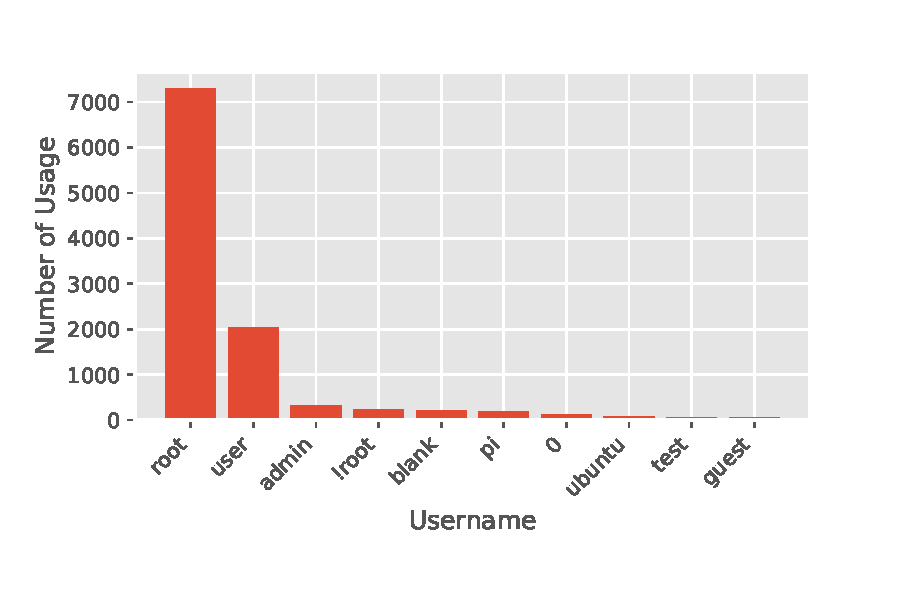
\includegraphics[width=\textwidth]{figures/tpot-cowrie-username.pdf}
        \caption{Cowrie username credentials}
        \label{fig:tpot-cowrie-username}
    \end{subfigure}
    \hfill
    \begin{subfigure}[b]{0.49\textwidth}
        \centering
        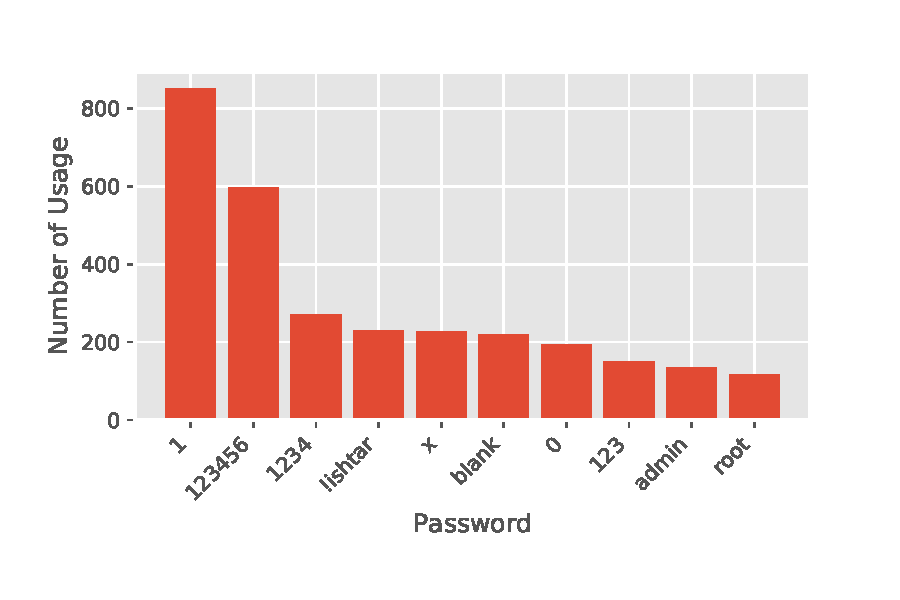
\includegraphics[width=\textwidth]{figures/tpot-cowrie-password.pdf}
        \caption{Cowrie password credentials}
        \label{fig:tpot-cowrie-password}
    \end{subfigure}
    \caption[Cowrie top 10 credentials on T-Pot]{
        Cowrie top 10 credentials used on T-Pot.
        Timestamp; 26th of September to 16th of October.
    }
    \label{fig:cowrie-credentials}
\end{figure*}

% ====================================================================================================================
% P0f
P0f identified different Windows versions and Linux distributions in conjunction with various \ac{ssh} clients to compromise the T-Pot.
Like \citet{Kelly2021}, Windows 7 or 8 and Windows NT Kernel are the most used \ac{os} with $81\%$.
Unfortunately, disguising OS fingerprinting activities account for $84\%$ of all fingerprints.
Lastly, the results are cleaned up and excluded all IPs from DFN and \acs{belwue} from the results.
Both scan frequently and check if any vulnerability exists.
This distorts the findings, and thus, they have been filtered based on their subnet addresses.
However, the results show no notable changes.
The total number of attacks was hardly influenced by it.
This indicates that these scans do not greatly interfere with the findings.

% ====================================================================================================================
% Conclusion
On average, heiCLOUD has received $55.83\%$ more than Azure, \ac{gcp}, and \ac{aws}.
Attacks on Cowrie, RDPY, and Honeytrap are the most compromised honeypots.
In contrast to \citet{Kelly2021}, Dionaea and Glutton used to be the most considered honeypots for adversaries.
It can be assumed that attacks by bots had increased significantly since last year when \citet{Kelly2021} did their research.
Respectively, one unresolved question is if other cloud providers filter their network traffic.
It would explain the major difference between Heidelberg University and the big tech companies.
The cause for such an increase remains doubtful.
One explanation could root back to the Corona pandemic and the skyrocketing increase in home office activities.
Related to that is a higher usage in screen sharing software.
Considering the BSI\footnote{The Federal Office for Information Security is responsible for managing communication security for the German government.
Each year they publish a report for recent cybersecurity threats.}, report for cybersecurity 2021 \cite{bsi2021}, they revealed an increase of attack surfaces during the pandemic.
Respectively, the IT infrastructure could not keep up with this fast change and widen the company's attack surface.
Their conclusion overlays our assumption that attackers took advantage and increased their activities.
This phenomenon shows that nearly all attacks originate from bots that scan through \ac{ip} address ranges.
In total, $73\%$ of all \ac{ip} addresses are unresolved.
The known attacker reputation represents the largest part of resolved \ac{ip} addresses with $23\%$.
Fortunately, such reputations could technically be filtered by an organization's firewall and would lower the chance of an exploit.
Interestingly, after three weeks, the number of attacks originating from China decreased to almost zero percent.
This might indicate that the honeypot has been exposed, and further attacks represent a risk of revealing their compromises.
However, this assumption cannot be confirmed due to the lax geographical reliability of \ac{ip} addresses.

Our results emphasize the importance of honeypots.
It gives a proper security measure of an IT infrastructure and helps to identify potential leaks or vulnerabilities.
Moreover, it shows that T-Pot helps detect recent bot activities and gives an outlook on the newest trends of attacks.

\begin{sidewaystable}
    \centering
    \caption[Overview of attacks on heiCLOUD, \ac{aws}, \ac{gcp}, and Azure]{
        Overview of attacks on heiCLOUD, \ac{aws}, \ac{gcp}, and Azure.
        Only the top 10 most attacked honeypots are considered.
        \enquote{-} entails that a honeypot is not part of the top 10.
        The red and green arrows indicate whether heiCLOUD received more or fewer attacks than the other cloud providers on average .
    }
    \begin{tabularx}{\linewidth}{l|rrc|rr|rr|rr}
        \toprule
        \textsc{Honeypots} & \multicolumn{3}{c}{BASIS}              & \multicolumn{6}{c}{\textsc{comparison}}                                                                                                                                                                 \\
                           & \multicolumn{3}{c|}{\textsc{heiCLOUD}} & \multicolumn{2}{c|}{\textsc{\ac{aws}}}       & \multicolumn{2}{c|}{\textsc{GC}} & \multicolumn{2}{c}{\textsc{Azure}}                                                                                         \\
                           & \textbf{Number}                        & \textbf{Pct.}                           &                                  & \textbf{Number}                    & \textbf{Pct.} & \textbf{Number}   & \textbf{Pct.} & \textbf{Number}   & \textbf{Pct.} \\
        \hline
        ADBHoney           & \numprint{9302}                        & $1.65\%$                                & $\color{green}{\uparrow}$        & \numprint{413}                     & $0.17\%$      & \numprint{2497}   & $0.43\%$      & \numprint{442}    & $0.13\%$      \\
        Cisco ASA          & \numprint{674}                         & $0.11\%$                                & $\color{green}{\uparrow}$        & \numprint{260}                     & $0.10\%$      & \numprint{750}    & $0.13\%$      & \numprint{134}    & $0.04\%$      \\
        Citrix honeypot    & \numprint{1121}                        & $0.18\%$                                &                                  & -                                  & -             & -                 & -             & -                 & -             \\
        Conpot             & \numprint{615}                         & $0.10\%$                                &                                  & -                                  & -             & -                 & -             & -                 & -             \\
        Cowrie             & \numprint{75511}                       & $11.97\%$                               & $\color{red}{\downarrow}$        & \numprint{4503}                    & $1.81\%$      & \numprint{297818} & $51.25\%$     & \numprint{9,012}  & $2.64\%$      \\
        DDoSPot            & \numprint{0}                           & $0\%$                                   &                                  & -                                  & -             & -                 & -             & -                 & -             \\
        Dicompot           & \numprint{22}                          & $0\%$                                   &                                  & -                                  & -             & -                 & -             & -                 & -             \\
        Dionaea            & \numprint{2368}                        & $0.40\%$                                & $\color{red}{\downarrow}$        & \numprint{228075}                  & $91.91\%$     & \numprint{162570} & $27.98\%$     & \numprint{308102} & $90.42\%$     \\
        Elasticpot         & \numprint{385}                         & $0.06\%$                                &                                  & -                                  & -             & -                 & -             & -                 & -             \\
        Glutton            & \numprint{0}                           & $0\%$                                   & $\color{red}{\downarrow}$        & \numprint{11878}                   & $4.79\%$      & \numprint{84375}  & $15.52\%$     & \numprint{17256}  & $5.06\%$      \\
        Heralding          & \numprint{35680}                       & $4.34\%$                                & $\color{green}{\uparrow}$        & \numprint{1885}                    & $0.76\%$      & \numprint{12,255} & $2.11\%$      & \numprint{3370}   & $0.99\%$      \\
        HoneyPy            & \numprint{0}                           & $0\%$                                   & $\color{red}{\downarrow}$        & \numprint{172}                     & $0.07\%$      & \numprint{2149}   & $0.37\%$      & \numprint{497}    & $0.15\%$      \\
        HoneySAP           & \numprint{15}                          & $0\%$                                   &                                  & -                                  & -             & -                 & -             & -                 & -             \\
        Honeytrap          & \numprint{201949}                      & $32.01\%$                               &                                  & -                                  & -             & -                 & -             & -                 & -             \\
        IPPHoney           & \numprint{0}                           & $0\%$                                   &                                  & -                                  & -             & -                 & -             & -                 & -             \\
        Mailoney           & \numprint{0}                           & $0\%$                                   & $\color{red}{\downarrow}$        & \numprint{720}                     & $0.29\%$      & \numprint{9419}   & $1.62\%$      & \numprint{146}    & $0.04\%$      \\
        MEDpot             & \numprint{2}                           & $0\%$                                   &                                  & -                                  & -             & -                 & -             & -                 & -             \\
        RDPY               & \numprint{280040}                      & $49.15\%$                               & $\color{green}{\uparrow}$        & \numprint{100}                     & $0.04\%$      & \numprint{7916}   & $1.36\%$      & \numprint{1463}   & $0.43\%$      \\
        SNARE/TANNER       & \numprint{63}                          & $0.02\%$                                & $\color{red}{\downarrow}$        & \numprint{138}                     & $0.06\%$      & \numprint{1367}   & $0.24\%$      & \numprint{313}    & $0.09\%$      \\
        \hline
        \textsc{In total}  & \numprint{607747}                      & $100\%$                                 &                                  & \numprint{248144}                  & $100\%$       & \numprint{581116} & $100\%$       & \numprint{340735} & $100\%$       \\
        \bottomrule
    \end{tabularx}
    \label{tab:overview-honeypots-attacks}
\end{sidewaystable}

\section{Discussion}

One downside of T-Pot is the static hostname representation of Cowrie.
It always returns \verb|#1 SMP Debian 3.2.68-1+deb7u1| (\verb|uname -a|) as hostname information, leaving a tiny footprint when bots crawl through the web.
A random choice of hostname information could harden Cowrie from being exposed.
Next, if attackers scan open ports on T-Pot, it might be suspicious when many ports with services are open.
From a technical perspective, bots could check this state if it is uncommon and thus, exclude T-Pot from being probed.
However, T-Pot includes reasonable preventions like a random hostname and scheduled tasks.
Another major drawback is the latest endeavor to detect honeypots on the transport level.
As recently investigated by \citet{vetterl2020}, detecting honeypots is becoming easier due to a fatal flaw in the underlying protocol implementation.
\citet{vetterl2020} states that attackers always try to prevent their methods, exploits, and tools from being divulged.
Therefore, detecting honeypots before attacking them strongly motivates black hats.
The \autoref{chap:fingerprinting} will present a way to avoid such fingerprint activities with the honeypot Cowrie.
